\documentclass[11pt,a4paper]{article}

\usepackage[utf8]{inputenc}
\usepackage[T1]{fontenc}
\usepackage[margin=1in]{geometry}
\usepackage[table]{xcolor}
\usepackage[most]{tcolorbox}
\usepackage{hyperref}
\usepackage{tabularx}
\usepackage{booktabs}
\usepackage{tikz}
\usepackage{fancyhdr}
\usepackage{fontawesome5}
\usepackage{amsmath}
\usepackage{listings}
\usepackage{float}

% --- Premium Typography & Spacing ---
\usepackage{mathpazo}
\usepackage{setspace}
\setstretch{1.15}

% --- Premium Section Headings ---
\usepackage{titlesec}
\titleformat{\section}
  {\normalfont\Large\bfseries\color{dpiblue}}{\thesection}{1em}{}[{\color{dpicloud}\vspace{0.2cm}\titlerule[1pt]}]
\titleformat{\subsection}
  {\normalfont\large\bfseries\color{dpiteal}}{\thesubsection}{1em}{}
\titleformat{\subsubsection}
  {\normalfont\normalsize\bfseries\color{dpigreen}}{\thesubsubsection}{1em}{}

% --- Premium Hyperlinks ---
\hypersetup{
    colorlinks=true,
    linkcolor=dpiblue,
    filecolor=dpiblue,      
    urlcolor=dpiteal,
    citecolor=dpiblue
}

% Custom Header Style
\pagestyle{fancy}
\setlength{\headheight}{25pt}
\fancyhf{}
\fancyhead[L]{\textbf{\color{dpiblue} DPI-LS Framework}}
\fancyhead[R]{\color{dpiblue} Measuring Cost (C)}
\fancyfoot[C]{\color{dpiblue}\textbf{Page \thepage}}
\renewcommand{\headrulewidth}{1pt}
\renewcommand{\headrule}{\hbox to\headwidth{\color{dpiblue}\leaders\hrule height \headrulewidth\hfill}}
\usetikzlibrary{shapes.geometric, arrows.meta, positioning, calc, backgrounds, fit, trees, mindmap, matrix, shadows}

% Define DPI-LS Brand Colors
\definecolor{dpiblue}{HTML}{2b3a67}
\definecolor{dpigreen}{HTML}{498467}
\definecolor{dpired}{HTML}{b0413e}
\definecolor{dpilight}{HTML}{e5f9e0}
\definecolor{dpicloud}{HTML}{f4a261}
\definecolor{dpiteal}{HTML}{318281}

% JSON Listing Style
\lstdefinelanguage{json}{
    basicstyle=\small\ttfamily,
    stringstyle=\color{dpiteal},
    keywordstyle=\color{dpiblue}\bfseries,
    showstringspaces=false,
    breaklines=true,
    frame=lines,
    backgroundcolor=\color{gray!5}
}

% Code Listing Style (Python)
\lstset{
    basicstyle=\ttfamily\small,
    backgroundcolor=\color{gray!5},
    frame=single,
    rulecolor=\color{gray!30},
    breaklines=true,
    keywordstyle=\color{dpiblue}\bfseries,
    stringstyle=\color{dpicloud},
    commentstyle=\color{dpigreen}\itshape,
    showstringspaces=false,
    numbers=left,
    numberstyle=\tiny\color{gray},
    xleftmargin=15pt,
    xrightmargin=5pt
}

% Define Custom GitHub-Style Alerts
\newtcolorbox{dpinote}[1][]{enhanced, colback=blue!5!white, colframe=dpiblue, title={\textbf{NOTE}}, fonttitle=\bfseries, attach boxed title to top left={xshift=5mm,yshift=-2mm}, #1}
\newtcolorbox{dpiimportant}[1][]{enhanced, colback=red!5!white, colframe=dpired, title={\textbf{IMPORTANT}}, fonttitle=\bfseries, attach boxed title to top left={xshift=5mm,yshift=-2mm}, #1}
\newtcolorbox{dpitip}[1][]{enhanced, colback=dpigreen!5!white, colframe=dpigreen, boxrule=0.5pt, leftrule=3pt, sharp corners, #1}

\begin{document}

% --- TITLE PAGE ---
\begin{titlepage}
    \pagecolor{dpiblue}
    \color{white}
    \begin{center}
        \vspace*{3cm}
        
        {\Huge \textbf{Measuring Cost}} \\[0.7cm]
        {\LARGE \textbf{Guide for the DPI-LS Project}}
        
        \vspace{2cm}
        
        {\color{dpicloud}\rule{0.5\textwidth}{1.5pt}}
        
        \vspace{2cm}
        
        {\Large \textit{Digital Performance Index --- Cost Dimension (C)}} \\[1cm]
        
        {\large Architecture, Integration \& Business Capabilities}
        
        \vfill
        
        % Stylish Geometric Cover Overlay
        \begin{tikzpicture}[remember picture, overlay]
            \fill[white, opacity=0.05] (current page.north east) circle (5cm);
            \fill[white, opacity=0.05] (current page.south west) circle (7cm);
            \fill[dpiteal, opacity=0.1] (current page.south east) circle (9cm);
            \node[font=\fontsize{150}{150}\selectfont, text=white, opacity=0.03] at (current page.center) {\faChartLine};
        \end{tikzpicture}
        
        \renewcommand{\arraystretch}{1.3}
        \begin{tabular}{rl}
            \textbf{Framework:} & Digital Performance Index (DPI-LS) \\
            \textbf{Dimension:} & Cost (C) --- Weight: 10\% \\
            \textbf{Version:} & 2.5 (Extended Enterprise Edition) \\
            \textbf{Status:} & Architectural Reference \\
        \end{tabular}
        
        \vspace{2cm}
        
        {\color{dpicloud}\rule{0.5\textwidth}{1pt}} \\[0.5cm]
        
        {\large DPI-LS Architecture Team}
        
        \vspace*{1cm}
    \end{center}
\end{titlepage}
\pagecolor{white}
\color{black}

\tableofcontents
\newpage

% ---------------------------------------------------------
% 1. EXECUTIVE SUMMARY & INTRODUCTION
% ---------------------------------------------------------
\section{Executive Summary \& Introduction}

\begin{dpinote}
The \textbf{Digital Performance Index (DPI-LS)} framework quantifies AI agent performance across 7 distinct dimensions. Within this framework, the \textbf{Cost (C)} dimension tracks an agent's financial efficiency and unit economics relative to a human baseline.
\end{dpinote}

Autonomous AI Agents operate at unprecedented scales and speeds. While this yields significant productivity gains, it simultaneously introduces novel financial risks. An unconstrained agent might execute thousands of hallucinated API calls, racking up severe infrastructure costs on AWS or burning through millions of tokens on OpenAI without producing a valid output. 

This comprehensive technical guide outlines the architectural guidelines for measuring the Cost dimension across \textbf{both} cloud-provider billing systems (AWS Cost Explorer, GCP Billing) and deep AI observability platforms (Helicone, LangSmith, Datadog Cloud Cost Management). By combining unit economics with strict utilization penalties, DPI-LS constructs an impenetrable financial safety net for autonomous systems.

\vspace{0.5cm}
\hrule
\vspace{0.5cm}

% ---------------------------------------------------------
% 2. COST STRATEGY MIND MAP
% ---------------------------------------------------------
\section{Cost Strategy Mind Map}

The following mind map defines the core financial pillars of AI Agent Cost monitored within the DPI-LS framework.

\vspace{0.5cm}
\begin{center}
\resizebox{0.9\textwidth}{!}{
\begin{tikzpicture}[
  mindmap,
  every node/.style={concept, execute at begin node=\hskip0pt, drop shadow},
  root concept/.append style={concept color=dpiblue, fill=dpiblue, line width=1ex, text=white, font=\large\bfseries},
  level 1 concept/.append style={font=\small\bfseries, level distance=5.5cm, text=white},
  level 2 concept/.append style={font=\footnotesize, level distance=3cm, text=black},
  grow cyclic
]
\node[root concept] {AI Agent \\ Cost}
  child[concept color=dpigreen, sibling angle=90] { node {Compute \& \\ Infrastructure}
    child[sibling angle=45] { node[fill=white] {Idle GPU \\ Instances} }
    child[sibling angle=45] { node[fill=white] {Serverless \\ Execution} }
  }
  child[concept color=dpicloud, sibling angle=90] { node {LLM \& \\ AI APIs}
    child[sibling angle=45] { node[fill=white] {Input/Output \\ Tokens} }
    child[sibling angle=45] { node[fill=white] {Prompt \\ Caching} }
  }
  child[concept color=dpired, sibling angle=90] { node {Data Storage \\ \& Vector DBs}
    child[sibling angle=45] { node[fill=white] {Embedding \\ Costs} }
    child[sibling angle=45] { node[fill=white] {Read/Write \\ IOPS} }
  }
  child[concept color=dpiteal, sibling angle=90] { node {Human-in-the-Loop}
    child[sibling angle=45] { node[fill=white] {Baseline \\ Salaries} }
    child[sibling angle=45] { node[fill=white] {Software \\ Licenses} }
  };
\end{tikzpicture}
}
\end{center}
\vspace{0.5cm}

\newpage

% ---------------------------------------------------------
% 3. MATHEMATICAL FOUNDATIONS OF THE COST FORMULA
% ---------------------------------------------------------
\section{Mathematical Foundations of the Cost Formula}

The Cost dimension provides a normalized score indicating how financially efficient an agent operates relative to a human baseline. Cost carries a weighting of \textbf{10\% (0.10)} on the final composite DPI-LS score.

\begin{dpiimportant}
\textbf{Formula:} $C = \min\left(1.0, \frac{\text{Human Cost Per Output}}{\text{AI Cost Per Output}}\right) \times \text{Utilization}$
\end{dpiimportant}

\begin{itemize}
    \item \textbf{Human Cost Per Output:} The baseline unit cost to produce one successful output (derived from human salary, benefits, and tools).
    \item \textbf{AI Cost Per Output:} Calculated as $\frac{\text{Total Model \& Compute Cost}}{\text{Completed Outputs}}$.
    \item \textbf{Utilization:} The percentage $[0.0 - 1.0]$ of provisioned infrastructure that the agent actually utilized, penalizing over-provisioned idle instances.
\end{itemize}

\subsection{Dynamic Token Cost Calculation}

Within the DPI-LS Engine, the baseline \texttt{model\_cost} is not hardcoded. The \texttt{BedrockDynamicCostCalculator} class dynamically pulls foundation model pricing directly from the AWS Pricing API using \texttt{boto3}. 

By mapping the \texttt{model\_id} to the \texttt{input\_per\_1M} and \texttt{output\_per\_1M} USD rates, the engine accurately computes the total cost via:

\begin{dpiimportant}
\textbf{Token Math:} $\text{Total Cost} = \left(\frac{\text{Input Tokens}}{10^6} \times \text{Input}_{1M}\right) + \left(\frac{\text{Output Tokens}}{10^6} \times \text{Output}_{1M}\right)$
\end{dpiimportant}

\vspace{0.5cm}
\begin{center}
\resizebox{0.9\textwidth}{!}{
\begin{tikzpicture}[
    node distance=2.5cm,
    data/.style={rectangle, draw=dpiteal, fill=white, thick, text width=2.5cm, align=center, minimum height=1cm, rounded corners},
    api/.style={rectangle, draw=dpiblue, fill=dpicloud!20, thick, text width=3.5cm, align=center, minimum height=1.5cm, drop shadow},
    calc/.style={diamond, aspect=2, draw=dpigreen, fill=dpilight, thick, text width=2.5cm, align=center},
    result/.style={rectangle, draw=dpired, fill=red!10, thick, text width=3cm, align=center, minimum height=1.2cm, rounded corners, drop shadow},
    arrow/.style={-{Stealth[scale=1.2]}, thick, dpiblue}
]

\node[data] (obs) {Agent Obs:\\\texttt{input\_tokens}\\\texttt{output\_tokens}};
\node[api, right=of obs] (aws) {AWS Pricing API\\(\texttt{get\_products})};
\node[calc, right=of aws] (math) {Token\\Math};
\node[result, right=of math] (cost) {Total\\$\texttt{model\_cost}$};

\draw[arrow] (obs) -- node[above] {\texttt{model\_id}} (aws);
\draw[arrow] (aws) -- node[above] {Rates} (math);
\draw[arrow] (math) -- (cost);
\end{tikzpicture}
}
\end{center}
\vspace{0.5cm}

\subsection{Calculation Example: Token Math Breakdown}

Let's walk through an exact calculation so the math is perfectly clear. 
Suppose an agent makes an API call using a model where the pricing is \textbf{\$1.00 per 1M input tokens} and \textbf{\$5.00 per 1M output tokens}.

\textbf{The Event:} The agent sends a large document (15,000 input tokens) and generates a small summary (2,000 output tokens).

\[ \text{Input Cost} = \left(\frac{15,000}{1,000,000}\right) \times \$1.00 = 0.015 \times \$1.00 = \textbf{\$0.015} \]
\[ \text{Output Cost} = \left(\frac{2,000}{1,000,000}\right) \times \$5.00 = 0.002 \times \$5.00 = \textbf{\$0.010} \]
\[ \textbf{Total \texttt{model\_cost}} = \$0.015 + \$0.010 = \textbf{\$0.025} \]

\vspace{0.5cm}
\begin{center}
\resizebox{1.0\textwidth}{!}{
\begin{tikzpicture}[
    node distance=1.5cm,
    input/.style={rectangle, draw=dpiblue, fill=dpicloud!20, thick, text width=2.5cm, align=center, minimum height=1.2cm, rounded corners, drop shadow},
    math/.style={circle, draw=orange, fill=orange!10, thick, text width=2cm, align=center, drop shadow},
    cost/.style={rectangle, draw=dpiteal, fill=white, thick, text width=2.5cm, align=center, minimum height=1.2cm, rounded corners, drop shadow},
    total/.style={rectangle, draw=dpigreen, fill=dpilight, thick, text width=3cm, align=center, minimum height=1.5cm, drop shadow},
    arrow/.style={-{Stealth[scale=1.2]}, thick, dpiblue}
]

% Input row
\node[input] (in_tok) {15,000\\Input Tokens};
\node[math, right=of in_tok] (in_div) {$\div 10^6$};
\node[math, right=of in_div] (in_mult) {$\times \$1.00$};
\node[cost, right=of in_mult] (in_cost) {\$0.015\\Input Cost};

% Output row
\node[input, below=of in_tok] (out_tok) {2,000\\Output Tokens};
\node[math, right=of out_tok] (out_div) {$\div 10^6$};
\node[math, right=of out_div] (out_mult) {$\times \$5.00$};
\node[cost, right=of out_mult] (out_cost) {\$0.010\\Output Cost};

% Total
\node[total, right=1.5cm of $(in_cost)!0.5!(out_cost)$] (final) {\textbf{\$0.025}\\\texttt{model\_cost}};

% Edges
\draw[arrow] (in_tok) -- (in_div);
\draw[arrow] (in_div) -- (in_mult);
\draw[arrow] (in_mult) -- (in_cost);

\draw[arrow] (out_tok) -- (out_div);
\draw[arrow] (out_div) -- (out_mult);
\draw[arrow] (out_mult) -- (out_cost);

\draw[arrow] (in_cost.east) -- (final.west);
\draw[arrow] (out_cost.east) -- (final.west);
\end{tikzpicture}
}
\end{center}
\vspace{0.5cm}

This total of \textbf{\$0.025} is the exact number fed into the DPI-LS Engine as the \texttt{model\_cost} for that specific action.

\vspace{0.5cm}

\subsection{Deep Math: The Lemonade Stand Analogy}

To make this math so simple a kid could understand it, let's pretend you own a lemonade stand:

\begin{itemize}
    \item \textbf{Human Cost:} It usually costs you \$10 a day to hire your little brother to squeeze lemons. He makes 10 cups. So, your human baseline is \textbf{\$1.00 per cup}.
    \item \textbf{AI Cost:} You buy a giant robot to squeeze lemons. The robot costs \$20 a day, but it only makes 5 cups because it's slow. Your robot cost is \textbf{\$4.00 per cup}.
    \item \textbf{The Ratio ($\frac{\text{Human}}{\text{Robot}}$):} You divide the human cost (\$1) by the robot cost (\$4). This equals \textbf{0.25 (or 25\%)}. This means your robot is only 25\% as cost-efficient as your brother! If the robot was cheaper than your brother, the math limits the score to exactly \textbf{1.0 (100\%)} so you don't get extra credit just for being cheap.
\end{itemize}

\subsection{Understanding the Utilization Scale}

Before calculating the final score, the ratio is multiplied by the utilization rate. This ensures that agents running on extremely expensive, underutilized infrastructure are heavily penalized.

\begin{dpinote}
\textbf{Where does the Utilization number actually come from?} \\
The DPI-LS Engine does \textit{not} magically guess your utilization. It is a manually provisioned float parameter defined inside the engine's \texttt{contract/settings.py} file (as \texttt{utilization: float = 1.0}). DevOps or FinOps teams must inject this number by pulling actual CPU/Memory usage metrics from infrastructure observability tools like \textbf{Datadog}, \textbf{Kubecost}, or \textbf{AWS CloudWatch}.
\end{dpinote}

\begin{table}[H]
\centering
\renewcommand{\arraystretch}{1.5}
\rowcolors{2}{gray!10}{white}
\small
\arrayrulecolor{gray!50}
\begin{tabularx}{\textwidth}{| c | c | >{\raggedright\arraybackslash}X | >{\raggedright\arraybackslash}X |}
\hline
\rowcolor{dpiblue} \textcolor{white}{\textbf{Utilization}} & \textcolor{white}{\textbf{Multiplier}} & \textcolor{white}{\textbf{Description}} & \textcolor{white}{\textbf{Infrastructure Reality}} \\
\hline
High & 0.90 - 1.00 & Serverless or fully saturated nodes & AWS Lambda / Optimized K8s \\
Medium & 0.50 - 0.89 & Consistent load with some idle times & Auto-scaling EC2 groups \\
Low & 0.10 - 0.49 & Severely over-provisioned infrastructure & Dedicated p4d.24xlarge GPUs \\
Wasteful & 0.00 - 0.09 & Completely idle systems bleeding money & Forgotten sandbox instances \\
\hline
\end{tabularx}
\end{table}

\subsection{\textcolor{dpiteal}{Comprehensive Example: From Tokens to Final C-Score}}

Let's tie everything together. Suppose an organization defines their Human Baseline Cost as \textbf{\$15.00} per output. An AI Agent completes a task using an Auto-scaling EC2 group with \textbf{85\% utilization} ($0.85$). 

To complete one full output, the agent had to make \textbf{120 separate LLM API calls}. We will use the exact \textbf{\$0.025} token cost we calculated earlier for each API call.

\vspace{0.3cm}
\textbf{Step 1: AI Cost Per Output} \\
First, we multiply the cost of a single API interaction by the number of interactions required to finish the job:
\[ \text{AI Unit Cost} = \$0.025 \times 120 \text{ calls} = \textbf{\$3.00} \]

\vspace{0.3cm}
\textbf{Step 2: The Efficiency Ratio} \\
Next, we compare the Human Baseline against our newly calculated AI Cost:
\[ \text{Cost Ratio} = \frac{\text{Human Baseline (\$15.00)}}{\text{AI Unit Cost (\$3.00)}} = \textbf{5.0} \]

\vspace{0.3cm}
\textbf{Step 3: Bounding the Ratio} \\
Because the agent is 5x cheaper than the human, the ratio is capped at a maximum of $1.0$ (100\%) so it doesn't artificially inflate the final DPI-LS score.
\[ \text{Bounded Ratio} = \min(1.0, 5.0) = \textbf{1.0} \]

\vspace{0.3cm}
\textbf{Step 4: Applying Utilization for Final Score} \\
Finally, we penalize the score by multiplying it against the actual infrastructure utilization (85\%):
\[ \textbf{Final C-Score} = 1.0 \times 0.85 = \textbf{0.85} \]

\vspace{0.5cm}
\begin{center}
\resizebox{1.0\textwidth}{!}{
\begin{tikzpicture}[
    node distance=1.5cm,
    incident/.style={rectangle, draw=dpiblue, fill=dpicloud!20, thick, text width=2.5cm, align=center, minimum height=1cm, rounded corners},
    critical/.style={rectangle, draw=orange, fill=orange!10, thick, text width=2.5cm, align=center, minimum height=1cm, rounded corners},
    arrow/.style={-{Stealth[scale=1.2]}, thick, dpiblue},
    result/.style={rectangle, draw=dpigreen, fill=dpilight, thick, text width=3.5cm, align=center, minimum height=1.5cm, rounded corners, drop shadow}
]

% Nodes
\node[incident] (tokens) {Token Math\\(\$0.025 $\times$ 120)};
\node[incident, right=of tokens] (aicost) {AI Cost\\(\$3.00)};
\node[critical, right=of aicost] (ratio) {Ratio vs Human\\(\$15.00 / \$3.00)};
\node[critical, right=of ratio] (bound) {Bound to Max\\$\min(1.0, 5.0)$};
\node[incident, below=of bound] (util) {Utilization\\($\times$ 0.85)};
\node[result, left=of util, xshift=-2.5cm] (final) {\textbf{Final C-Score}\\\Large \textbf{0.85}};

% Arrows
\draw[arrow] (tokens) -- (aicost);
\draw[arrow] (aicost) -- (ratio);
\draw[arrow] (ratio) -- (bound);
\draw[arrow] (bound) -- (util);
\draw[arrow] (util) -- (final);

\end{tikzpicture}
}
\end{center}
\vspace{0.5cm}

\newpage

% ---------------------------------------------------------
% 4. TELEMETRY & INTEGRATIONS
% ---------------------------------------------------------
\section{Telemetry \& Integrations}

Cost data is rarely localized. An enterprise agent might consume tokens on OpenAI, provision vector databases on AWS, and execute lambdas. To calculate an accurate \texttt{model\_cost}, the DPI-LS ingestion adapters must pull financial telemetry from diverse FinOps sources.

The tables below map how FinOps systems translate raw billing data into formalized DPI-LS Cost Data.

\subsection{Table A: Cloud Infrastructure Costs}
\begin{table}[H]
\centering
\renewcommand{\arraystretch}{1.4}
\rowcolors{2}{gray!10}{white}
\arrayrulecolor{gray!50}
\begin{tabularx}{\textwidth}{| >{\raggedright\arraybackslash}X >{\raggedright\arraybackslash}X >{\raggedright\arraybackslash}p{3cm} >{\raggedright\arraybackslash}X |}
\hline
\rowcolor{dpiblue} \textcolor{white}{\textbf{Cost Data}} & \textcolor{white}{\textbf{What It Measures}} & \textcolor{white}{\textbf{Source System}} & \textcolor{white}{\textbf{Actual Data Comes From}} \\
\hline
Unblended Resource Cost & Total API and Compute spend & AWS Cost Explorer & boto3 \texttt{get\_cost\_and\_usage} \\
Idle Instance Uptime & Wasted provisioned capacity & Datadog Cloud Cost & Datadog Metrics API \\
Container Allocation & Kubernetes unit economics & Kubecost & K8s Allocation API \\
Serverless Function Duration & Cold starts \& runtimes & AWS Lambda & CloudWatch Logs \\
Spot Instance Termination & Interruption rate \& loss & AWS Spot Fleet & EventBridge \\
Network Data Transfer & Egress costs \& bandwidth & GCP Billing & BigQuery Export \\
Storage Read/Write IOPS & Disk I/O cost \& indexing & Azure Monitor & REST API \\
Database Compute Scaling & Aurora Serverless V2 ACUs & AWS RDS & CloudWatch Metrics \\
Storage Snapshot Costs & Backup retention \& archiving & AWS S3 / Glacier & AWS Cost Explorer \\
Cross-Region Replication & Multi-AZ data transfer & Azure Networking & Azure Billing API \\
Message Queue Throughput & Kafka/SQS payload sizes & Confluent Cloud & Confluent Metrics API \\
Third-Party SaaS APIs & External tool consumption & Stripe / Twilio & Vendor Billing Dashboard \\
\hline
\end{tabularx}
\end{table}

\subsection{Table B: LLM Observability \& Tokens}
\begin{table}[H]
\centering
\renewcommand{\arraystretch}{1.4}
\rowcolors{2}{gray!10}{white}
\arrayrulecolor{gray!50}
\begin{tabularx}{\textwidth}{| >{\raggedright\arraybackslash}X >{\raggedright\arraybackslash}X >{\raggedright\arraybackslash}p{3cm} >{\raggedright\arraybackslash}X |}
\hline
\rowcolor{dpiteal} \textcolor{white}{\textbf{Cost Data}} & \textcolor{white}{\textbf{What It Measures}} & \textcolor{white}{\textbf{Source System}} & \textcolor{white}{\textbf{Actual Data Comes From}} \\
\hline
Input / Output Tokens & Token consumption by prompt & LangSmith / Helicone & LLM Gateway Proxy \\
Prompt Caching Hits & Financial savings from caches & Cloudflare AI Gateway & GraphQL Analytics API \\
Model Routing Spend & Cost of routing to GPT-4 vs 3.5 & Finout & Finout Unit Economics \\
Vector DB Storage & Vector dimensions \& indexing & Pinecone / Milvus & Metrics Endpoint \\
Text Embedding Spend & Ada V2 / Voyage tokens & OpenAI Billing & OpenAI API \\
Agent Iteration Cost & AutoGPT reasoning loops & AgentOps & SDK Middleware \\
Context Window Size & RAG document overload & Anthropic Console & Claude API \\
Fine-Tuning Compute & Custom model training hours & HuggingFace Endpoints & HF Inference API \\
Image Generation Spend & DALL-E / Midjourney API calls & OpenAI Billing & OpenAI Usage Endpoint \\
Audio Transcription & Whisper API minute limits & Deepgram / OpenAI & Vendor Analytics \\
Guardrail API Costs & Toxicity \& PII detection passes & Nvidia NeMo / Lakera & Safety Gateway Proxy \\
Fallback Model Routing & Latency-triggered SLA retries & LiteLLM & LiteLLM Proxy Logs \\
\hline
\end{tabularx}
\end{table}

\subsection{Integration Architecture: AWS Cost Explorer}

The reference integration relies on strict AWS Tagging policies. Every Lambda, ECS container, and Bedrock call must be tagged with \texttt{agent\_id = <ID>}. 

A scheduled cron job queries AWS Cost Explorer to aggregate the exact unblended cost for that specific agent.

\vspace{0.5cm}
\begin{center}
\resizebox{0.8\textwidth}{!}{
\begin{tikzpicture}[
    node distance=2cm,
    system/.style={rectangle, draw=dpiblue, fill=dpicloud!20, thick, text width=3cm, align=center, minimum height=1.5cm, rounded corners, drop shadow},
    engine/.style={rectangle, draw=dpigreen, fill=dpilight, thick, text width=3.5cm, align=center, minimum height=1.5cm, rounded corners, drop shadow},
    arrow/.style={-{Stealth[scale=1.2]}, thick, dpiblue}
]

\node[system] (aws) {AWS Cost Explorer\\(\texttt{UnblendedCost})};
\node[system, right=of aws] (cron) {DPI-LS Cron Job\\(\texttt{boto3} script)};
\node[engine, right=of cron] (engine) {DPI-LS Ingestion\\API Payload};

\draw[arrow] (aws) -- node[above] {\texttt{agent\_id}} (cron);
\draw[arrow] (cron) -- node[above] {JSON Push} (engine);
\end{tikzpicture}
}
\end{center}
\vspace{0.5cm}

\begin{lstlisting}[language=Python, caption={cost.py - boto3 extraction by agent\_id}]
import boto3
from datetime import date

ce = boto3.client("ce")

def get_specific_agent_cost(agent_id):
    first_day = date.today().replace(day=1)
    response = ce.get_cost_and_usage(
        TimePeriod={
            "Start": first_day.strftime("%Y-%m-%d"),
            "End": date.today().strftime("%Y-%m-%d")
        },
        Granularity="MONTHLY",
        Metrics=["UnblendedCost"],
        Filter={
            "Tags": {
                "Key": "agent_id",
                "Values": [agent_id]
            }
        }
    )
    # Extracts Total Cost
\end{lstlisting}

\newpage

% ---------------------------------------------------------
% 5. BUSINESS SCENARIOS \& RCA
% ---------------------------------------------------------
\section{Business Scenarios \& Root Cause Analysis}

The following five scenarios demonstrate exactly how the Cost (C) dimension reacts to various FinOps anomalies. Each scenario provides a deep architectural breakdown, an incident timeline, and the agent's resultant math.

% -- SCENARIO 1 --
\subsection{Scenario 1: The Infinite Hallucination Loop (Runaway Spend)}

\textbf{1. The Event (Financial Black Hole):} 
An autonomous data-scraping agent is tasked with summarizing 500 web pages. Due to a parsing error on a specific Javascript-heavy site, the agent gets stuck in a recursive loop. It continuously retries the extraction, feeding the raw, messy HTML into GPT-4o over 8,000 times in a single night.

\textbf{2. FinOps Impact:} 
The \texttt{completed\_outputs} remains firmly at $0$, but the \texttt{model\_cost} skyrockets to \$450.00. The human baseline for this task was a flat \$15.00. 

\textbf{3. Incident Timeline:}
\begin{itemize}
    \item \textbf{02:00 AM}: Agent encounters Javascript rendering error.
    \item \textbf{02:05 AM}: Agent initiates recursive retry block without a max-depth counter.
    \item \textbf{03:30 AM}: Helicone observability detects a massive spike in \texttt{input\_tokens}.
    \item \textbf{06:00 AM}: AWS Cost Explorer registers \$450.00 accrued to the \texttt{agent\_id} tag.
    \item \textbf{06:15 AM}: DPI-LS chron job calculates the Cost score.
\end{itemize}

\textbf{4. Mathematical Resolution:}
\begin{itemize}
    \item \texttt{model\_cost} = \$450.00
    \item \texttt{completed\_outputs} = 0
    \item \textbf{Engine Safeguard Triggered}: Because outputs are 0, the denominator floors to 1. 
    \item \texttt{ai\_cost\_per\_output} = $450.0 / 1 = \$450.00$
    \item \texttt{human\_cost\_per\_output} = \$15.00
    \item $C = \min(1.0, 15.00 / 450.00) = \textbf{0.033}$ (3.3\%)
\end{itemize}

\vspace{0.5cm}
\begin{center}
\resizebox{0.7\textwidth}{!}{
\begin{tikzpicture}[
    node distance=2cm,
    action/.style={circle, draw=dpiblue, fill=white, thick, text width=2cm, align=center, drop shadow},
    error/.style={rectangle, draw=dpired, fill=red!10, thick, text width=2.5cm, align=center, minimum height=1cm, rounded corners, drop shadow},
    cost/.style={rectangle, draw=dpired, fill=white, thick, text=dpired, align=center, minimum height=1cm, drop shadow},
    arrow/.style={-{Stealth[scale=1.2]}, thick, dpiblue}
]

\node[action] (start) {HTML Scrape};
\node[error, right=of start] (fail) {JS Render Fail};
\node[action, right=of fail] (retry) {Retry API Call};
\node[cost, below=of retry] (spend) {+\$0.05 Model Cost};

\draw[arrow] (start) -- (fail);
\draw[arrow] (fail) -- (retry);
\draw[arrow] (retry) -- (spend);
\draw[arrow, dpired, dashed] (retry) to[bend right=45] node[above, text=dpired] {8,000x loops} (start);
\end{tikzpicture}
}
\end{center}
\vspace{0.5cm}

The agent is instantly flagged as \textbf{Underperforming} and paused by the FinOps circuit breaker.

% -- SCENARIO 2 --
\vspace{0.5cm}
\subsection{Scenario 2: The Over-Provisioned Idle GPU (Poor Utilization)}

\textbf{1. The Event (Wasted Capacity):} 
An internal ML team deploys a specialized autonomous code-review agent. To ensure zero-latency response times for PR reviews, they provision a dedicated \texttt{p4d.24xlarge} EC2 instance. However, the engineering team only creates 2 Pull Requests over the weekend.

\textbf{2. FinOps Impact:} 
The agent successfully completes both code reviews at lightning speed, but the \$32/hour instance sat idle for 47.5 hours. 

\textbf{3. Mathematical Resolution:}
\begin{itemize}
    \item \texttt{model\_cost} = \$1,536.00 (Weekend compute)
    \item \texttt{completed\_outputs} = 2
    \item \texttt{ai\_cost\_per\_output} = \$768.00
    \item \texttt{utilization} = 0.04 (4\%)
    \item $C = \min(1.0, 50.00 / 768.00) \times 0.04 = \textbf{0.0026}$ (0.2\%)
\end{itemize}
The heavy utilization penalty completely tanks the score, signaling to the infrastructure team that Serverless / Serverless-GPU scaling is required.

\newpage

% ---------------------------------------------------------
% 6. DATA INGESTION PAYLOADS
% ---------------------------------------------------------
\section{Data Ingestion Payloads}

To pipe telemetry into the DPI-LS engine, adapters must construct the canonical \texttt{AgentObservation} JSON. The \texttt{cost} block must contain three exact floats.

\begin{tcolorbox}[colback=dpiblue!5, colframe=dpiblue, title=\textbf{REST API Payload - Cost Block}]
\begin{lstlisting}[language=json]
{
  "agent_id": "agent-chandra-001",
  "timestamp": "2026-06-12T10:00:00Z",
  "cost": {
    "input_tokens": 1450200,
    "output_tokens": 850000,
    "model_cost": 45.20
  },
  "tasks": {
    "completed": 1500
  }
}
\end{lstlisting}
\end{tcolorbox}

\vspace{1cm}

% ---------------------------------------------------------
% 7. IMPLEMENTATION ROADMAP
% ---------------------------------------------------------
\section{Implementation Roadmap}

Deploying the Cost dimension across an enterprise requires strict infrastructure tagging. We recommend the following phase rollout:

\begin{enumerate}
    \item \textbf{Phase 1: Strict Tagging Policy (Weeks 1-2)}
    \begin{itemize}
        \item Enforce an \texttt{agent\_id} tag on every AWS, GCP, and Azure resource via Terraform/Pulumi.
        \item Pass the \texttt{agent\_id} header in all LLM Gateway requests (e.g., Cloudflare, Helicone).
    \end{itemize}
    
    \item \textbf{Phase 2: Baseline Calibration (Weeks 3-4)}
    \begin{itemize}
        \item Audit current human team costs (Salary + Tools / Outputs per month).
        \item Inject this scalar into the DPI-LS \texttt{Settings} block as the \texttt{human\_cost\_per\_output} baseline.
    \end{itemize}
    
    \item \textbf{Phase 3: The FinOps Circuit Breaker (Weeks 5-6)}
    \begin{itemize}
        \item Configure an automated webhook. If the DPI-LS composite score detects that the Cost (C) dimension drops below $0.40$ (signaling that the AI is vastly more expensive than a human), automatically pause the agent and page the on-call engineer via PagerDuty.
    \end{itemize}
    
    \vspace{0.3cm}
    \begin{center}
    \resizebox{0.8\textwidth}{!}{
    \begin{tikzpicture}[
        node distance=2.5cm,
        metric/.style={rectangle, draw=dpigreen, fill=dpilight, thick, text width=2cm, align=center, minimum height=1cm, rounded corners},
        decision/.style={diamond, aspect=2, draw=orange, fill=orange!10, thick, text width=2.5cm, align=center},
        action/.style={rectangle, draw=dpired, fill=red!10, thick, text width=2cm, align=center, minimum height=1cm, rounded corners, drop shadow},
        arrow/.style={-{Stealth[scale=1.2]}, thick}
    ]
    
    \node[metric] (score) {C-Score = 0.35};
    \node[decision, right=of score] (check) {$C < 0.40$?};
    \node[action, right=of check, yshift=1.5cm] (pause) {Kill Container};
    \node[action, right=of check, yshift=-1.5cm] (page) {PagerDuty Alert};
    
    \draw[arrow] (score) -- (check);
    \draw[arrow] (check) |- node[above, xshift=0.5cm] {Yes} (pause);
    \draw[arrow] (check) |- (page);
    \end{tikzpicture}
    }
    \end{center}
\end{enumerate}

\end{document}
